\documentclass[11pt,letterpaper]{article}
\usepackage[T1]{fontenc}
\usepackage[utf8]{inputenc}
\usepackage{lmodern,microtype}
\usepackage[margin=1in,headheight=15pt]{geometry}
\usepackage{amsmath,amssymb,amsthm,mathtools}
\usepackage{graphicx,booktabs,longtable,array,enumitem}
\usepackage{xcolor}
\definecolor{ink}{HTML}{17324D}
\definecolor{accent}{HTML}{176B72}
\usepackage[colorlinks=true,linkcolor=ink,citecolor=accent,urlcolor=accent]{hyperref}
\hypersetup{pdftitle={Compressed Component Certificates and Quadratic Periodic Scheduling for Unknot Recognition},
pdfauthor={Research continuation prepared for Vladimir Reshetnikov},
pdfsubject={ProveIt: rigorous compressed-kernel improvements and a research program toward quasi-polynomial unknot recognition},
pdfkeywords={unknot recognition, normal surfaces, weighted AHT, interval orbits, certificates}}
\usepackage[nameinlink,noabbrev]{cleveref}
\usepackage{fancyhdr}
\pagestyle{fancy}
\fancyhf{}
\fancyhead[L]{\small Compressed component certificates}
\fancyhead[R]{\small ProveIt research continuation}
\fancyfoot[C]{\thepage}
\renewcommand{\headrulewidth}{0.3pt}
\usepackage{titlesec}
\usepackage{needspace,etoolbox}
\titleformat{\section}{\large\bfseries\color{ink}}{\thesection}{0.7em}{}
\titleformat{\subsection}{\normalsize\bfseries\color{ink}}{\thesubsection}{0.7em}{}
\pretocmd{\section}{\Needspace{6\baselineskip}}{}{}
\pretocmd{\subsection}{\Needspace{5\baselineskip}}{}{}
\setlength{\parskip}{0.32em}
\setlength{\parindent}{1.2em}
\setlist{itemsep=0.2em,topsep=0.4em}
\newtheorem{theorem}{Theorem}[section]
\newtheorem{lemma}[theorem]{Lemma}
\newtheorem{proposition}[theorem]{Proposition}
\newtheorem{corollary}[theorem]{Corollary}
\theoremstyle{definition}
\newtheorem{definition}[theorem]{Definition}
\newtheorem{remark}[theorem]{Remark}
\newcommand{\code}[1]{\texttt{#1}}
\newcommand{\Z}{\mathbb Z}
\newcommand{\Ftwo}{\mathbb F_2}
\newcommand{\poly}{\operatorname{poly}}
\newcommand{\polylog}{\operatorname{polylog}}
\newcommand{\baselinecommit}{\texttt{274909dd8724e411ece14e47ac4addea717aeca6}}
\title{\vspace{-1.6em}{\color{ink}\bfseries Compressed Component Certificates\\
and Quadratic Periodic Scheduling\\for Unknot Recognition}}
\author{Research continuation prepared for Vladimir Reshetnikov\\
\small ProveIt / Topology / UnknotRecognition}
\date{9 October 2026\\[-0.2em]\small Source snapshot: 8 October 2026, 20:25 PDT}
\begin{document}
\maketitle
\thispagestyle{empty}
\begin{abstract}
We extend ProveIt's binary normal-surface backend in two complementary ways.
First, we replace repeated all-pairs periodic-merger scans by a stable,
generation-checked event queue, with an adaptive prelude for easy instances.
The successful reductions and complete certificates are unchanged. A phase
with \(k\) pairings uses at most \((k-1)^2\) merger tests in queue mode and at
most \(\binom{k}{2}+(k-1)^2\) in adaptive mode. An explicit \(k=2m\) family
takes exactly five complete Agol--Hass--Thurston cycles: historical merger work
is \(m^3+(m^2+5m)/2-4\), whereas eager queue work is \(5m^2-6m+2\).
Second, we implement classical weighted orbit replay and construct five
integer weights that identify and count compressing-disk components inside a
possibly disconnected normal surface. The weights record Euler
characteristic, normal pieces, boundary vertices, and intersection counts
with a basis of torus boundary homology. This avoids explicit component
enumeration and does not require an orientation-double query for the disk
predicate. We give proofs, source-bound replay, independent finite oracles,
paired measurements, and a reproducible integration package.
These are improvements to a polynomial compressed kernel and to the
information it certifies. They do not supply the missing diagram-to-exterior
provenance, surface discovery, or compressed hierarchy needed for a general
quasi-polynomial unknot recognizer.
\end{abstract}
\vspace{0.4em}
\noindent\textbf{Research status.}
The scheduler theorem and its exact five-cycle lower-bound family are proved
here for the maintained algorithm. Weighted orbit computation is classical
AHT theory; the five-coordinate cellular construction is a focused
implementation of that theory. No claim of a new general complexity bound for
unknot recognition, or of priority for polynomial normal-surface topology, is made.
\clearpage
{\small\setlength{\parskip}{0pt}\tableofcontents}
\clearpage
\section{Objective, source audit, and the complexity target}
\label{sec:context}

The computational objective is to move the existing exact recognizer toward
an algorithm whose running time is bounded by
\(n^{(\log n)^{O(1)}}\), where \(n\) measures the input knot diagram. A useful
continuation must contribute an implemented step, a proved structural
bound, or a precisely exposed obstruction. Merely attaching a polynomial
subroutine to an exponential search does not settle this objective.

The present work targets compressed normal-surface analysis. A normal
surface can have exponentially many elementary disks while its coordinates
have only polynomially many bits. Thus a program that follows every normal
disk, every edge point, or every connected component explicitly is unsuitable
for the intended complexity target. The interval-pairing representation
already used by the repository is an appropriate starting point: its input
size is the number of pairings and the bit length of their endpoints.

\subsection{Pinned repository state}

All changes are relative to ProveIt commit
\begin{center}
\baselinecommit.
\end{center}
The \path{Topology/UnknotRecognition/fast} Git tree at that commit is
\begin{center}
\texttt{72834388419f5016d6db28ca0f028794f30b68db}.
\end{center}
The source was accessed through the selected GitHub connection. Locally
available copies were reused only after matching their Git blob contents to
the pinned tree; changed source files were fetched at the commit itself.
This distinction matters because the repository was receiving many concurrent
research integrations during the audit.

The maintained source contains substantially more than the original
Khovanov scanner. It includes compressed words and group certificates, braid
reductions, interval-component sharing, exact homological windows,
compressed twists, several Jones evaluators, and normal-surface topology
queries. We did not treat an old delivery snapshot as the current baseline.
The audit focused on
\path{fastunknot/interval_orbits.py},
\path{fastunknot/interval_orbit_verify.py},
\path{fastunknot/normal_surface_geometry.py}, and
\path{fastunknot/normal_surface_orbits.py}.
The corresponding maintained synthesis sections already explain interval
orbits, independent orbit proofs, coordinate multiplicity, and boundary
component classification \cite{ProveIt2026}.

Two limitations stand out in that source. Its periodic closure restarts a
lexicographic all-pairs search after every merge, even though only one
surviving pairing has changed. Its normal-surface topology query computes
aggregate Euler and component data, but its
\code{compressing\_disk} flag concerns the entire supplied surface being
a disk. The weighted component extraction needed to detect a disk hidden
inside a disconnected vector is explicitly absent.

The new work addresses these two limitations. It does not repeat the recent
compressed singleton-elimination or raw-contraction work on group
presentations. It also does not alter the meaning of the old
\code{compressing\_disk} field: a separate component query supplies the
stronger, differently quantified predicate.

\subsection{What the current literature establishes}

Agol, Hass, and Thurston proved polynomial-time counting for interval
pseudogroups, extended the algorithm to additive vector weights, and
applied it to compressed normal-surface components
\cite{AHT2006}. That classical result is the mathematical foundation of
the implementation here. In particular, the existence of a polynomial
algorithm for obtaining topology from supplied binary coordinates is not
a new theorem of this report.

The quasi-polynomial announcement must be stated with its actual
parameters. Lackenby's March 2021 Oxford handout gives
\[
 2^{O((\log n)^3)}
 =n^{O((\log n)^2)},
\]
with hierarchy length \(L=O((\log n)^2)\) and a polynomial surface-complexity
parameter \cite{Lackenby2021}. Earlier publicity used the stronger expression
\(n^{O(\log n)}\). Both are quasi-polynomial, but they are not identical
bounds and should not be substituted for one another in an implementation
claim.

Lackenby's July 2026 preprint gives a new hierarchy approach to
incompressibility and unknot recognition. Section 9 explicitly leaves the
running time of some operations unspecified; Proposition 9.1 bounds
iterations by \(L(g+1)^L\). Section 10 refines the hierarchy length, and
Theorem 14.4 treats compressed cutting and parallelity information
\cite{Lackenby2026}. These developments are highly relevant specifications
for future work, but the inspected preprint does not itself assert a
quasi-polynomial runtime for the full algorithm. The current repository
already records that qualification correctly.

\subsection{The deliverable's main statements}

The first result is an exact simulation theorem: the new scheduler produces
the same ordered sequence of successful periodic reductions as the pinned
implementation. It follows that all later carrier choices, transmissions,
truncations, and complete certificates agree as well. This is stronger than
merely observing equal final orbit counts.

The second result is a work bound that is independent of the expanded
interval size. A pure queue needs at most \((k-1)^2\) merger tests in one
closure. The adaptive default adds at most \(\binom{k}{2}\) preliminary
tests. The proof identifies precisely what is cached and what is invalidated;
it does not count failed arithmetic operations as free.

The third result exhibits a family on which the improvement changes
the asymptotic cost of a \emph{complete} count. Both old and new algorithms
take five cycles, so expensive later phases do not conceal the improvement.
This is an implementation-specific lower bound, not a lower bound for the
abstract orbit-counting problem.

The fourth result is a source-bound component predicate. Given a validated
compact orientable triangulation with one torus boundary and an admissible
normal vector, the new query counts all disk components and all
compressing-disk components without listing the components individually.
It uses five coordinates regardless of the triangulation size. This is
particularly useful when a candidate normal vector includes irrelevant
vertex links, closed components, or many parallel copies.

Throughout, \(k\) denotes an interval-pairing count, \(N\) its encoded
universe size, \(t\) a tetrahedron count, and \(n\) a knot-diagram size.
Bounds in \(k\) or \(t\) do not silently become bounds in \(n\). Any passage
between these parameters requires the corresponding geometric construction.

\section{Exact periodic scheduling with quadratic merger work}
\label{sec:queue}

\subsection{Interval pairings and the unchanged merger rule}

An interval pairing identifies the integer points of two intervals of equal
length by an isometry. We use inclusive endpoints in this section:
\[
 g:[a,b]\longrightarrow[c,d],\qquad a\le c,\quad b-a=d-c.
\]
The map is either \(x\mapsto x+c-a\) or the reflection
\(x\mapsto a+d-x\). A periodic pairing is an increasing pairing with
\(a<c\le b+1\). Its period is \(p=c-a>0\), and its support is \([a,d]\).
The convention includes two adjacent intervals.

For periodic pairings with periods \(p,q\), write \(h=\gcd(p,q)\).
The maintained sharp rule merges them when their support overlap has at least
\[
 p+q-h
\]
integer points. Their union is then represented by a period-\(h\)
pairing. This is the Fine--Wilf periodicity criterion in the form already
implemented and verified by the repository \cite{FineWilf1965,ProveIt2026}.
The alternative classical threshold \(p+q\) remains available. Our
scheduler uses the existing arithmetic test unchanged. The arguments below
about scheduling work for either rule.

The historical algorithm scans pairs of list indices in lexicographic order.
It accepts the first legal pair \((i,j)\), keeps the replacement at \(i\),
deletes \(j\), and restarts from the beginning. Since a merge changes only
one surviving row, most failed tests in the repeated prefix compare
unchanged data.

\subsection{Stable identifiers and generations}

Give each input row a permanent identifier equal to its original list
position. Active identifiers remain in increasing order when rows are
deleted. For each identifier keep a generation counter, initially zero.
Whenever a row is replaced, increment its counter. A heap entry contains
\[
 (i,j,\nu_i,\nu_j,\text{replacement}),
\]
ordered first by \(i\), then by \(j\). Its generations record the operands
on which the exact merger test was performed.

Initialisation tests every pair of periodic rows and inserts the successful
pairs. To perform a merge, discard stale heap minima until the first
current entry is found. An entry is stale when either identifier has
disappeared or either generation has changed. Replace the lower-identifier
row, remove the other, and test exactly the pairs incident to the
replacement. Entries for untouched pairs remain valid. No equality test
uses a fingerprint or a probabilistic hash.

\begin{theorem}[Exact simulation of the historical closure]
\label{thm:queue-exact}
For every finite ordered pairing list and either maintained periodic
threshold, the queue closure performs exactly the historical sequence of
successful merges. It returns the same ordered list. When it records current
list indices, its merger certificate is identical to the historical
certificate.
\end{theorem}
\begin{proof}
Maintain the following invariant: each legal current pair has exactly one
nonstale heap entry, and every nonstale entry is the correct successful test
on its present operands. Initialisation establishes the invariant.

Suppose it holds before a merge of \(i<j\). Pairs avoiding \(i,j\) have
unchanged operands, so both their legality and their existing entries are
unchanged. Deletion of \(j\) invalidates every entry involving \(j\).
Incrementing the generation of \(i\) invalidates all old entries involving
\(i\). Testing each surviving partner of the new \(i\) restores precisely
the missing current entries. The invariant is preserved.

The stable identifiers have the same relative order as current list
positions. The first nonstale heap entry is therefore the
lexicographically first legal pair of current rows, which is exactly the
historical choice. Induction proves equality of successful choices and
replacements. The rank of an identifier among active identifiers is its
current list index, giving the same certificate indices.
\end{proof}

The producer currently computes these ranks by scanning the active
identifiers. There are at most \(k-1\) mergers, so this adds \(O(k^2)\)
operations over a closure. A separate order-statistics structure would
complicate the implementation without improving its displayed asymptotic
bound.

\begin{corollary}[Complete trace preservation]
\label{cor:trace}
Replacing only periodic-closure scheduling in the maintained AHT routine
preserves the orbit count, the number of AHT cycles, and every complete
local-reduction certificate.
\end{corollary}
\begin{proof}
After each periodic closure the ordered pairing list is identical by
\cref{thm:queue-exact}. All subsequent carrier selection, maximal-power
transmission, suffix truncation, and next-cycle preparation are unchanged
deterministic operations on that list. Induct over the cycles.
\end{proof}

Callback invocation counts and scheduler work statistics are intentionally
not certificate contents. A wall-clock deadline can stop the algorithms at
different points because their costs differ. The corollary concerns
completed mathematical traces; a shared cycle cap still counts the same
begun AHT cycles.

\subsection{Work bound and the adaptive default}

\begin{theorem}[Quadratic candidate count]
\label{thm:queue-work}
For a closure starting with \(k\ge1\) rows, pure queue mode performs at most
\((k-1)^2\) exact merger tests. It requires at most \(O(k^2)\) heap entries.
For endpoint bit length \(B\), a conservative bit bound is
\[
 O\!\left(k^2\bigl(G(B)+B+\log^2(k+1)\bigr)\right),
\]
where \(G(B)\) bounds a gcd and the bounded number of endpoint operations
used in one merger test. The empty list requires no test.
\end{theorem}
\begin{proof}
Initialisation uses at most \(\binom{k}{2}\) tests. A merge leaving \(r\)
rows creates at most \(r-1\) incident candidates. Since the live row count
strictly decreases,
\[
 \binom{k}{2}+\sum_{r=1}^{k-1}(r-1)
 =\binom{k}{2}+\binom{k-1}{2}
 =(k-1)^2.
\]
Nonperiodic rows only reduce the number of candidates. Every successful
test inserts one entry; every entry can be popped at most once, including
stale entries. Thus the total heap size, insertions, and removals are
quadratic. Each heap operation takes \(O(\log(k+1))\) identifier
comparisons, on \(O(\log(k+1))\)-bit keys. Endpoint arithmetic and stored
replacement construction contribute the other terms. Rank scans and
output construction fit within the same bound.
\end{proof}

The storage bound in bits is \(O(k^2(B+\log(k+1)))\), excluding the input
and any separately retained full trace. This is a real tradeoff:
historical restarting needs only a linear working list.

Moreover, an eager queue is unnecessary on easy inputs. If every row is
identical, the historical closure succeeds immediately on its first pair
\(k-1\) times, whereas the queue begins by checking all
\(\binom{k}{2}\) pairs.

The adaptive default therefore first follows the historical candidate
sequence. At each restart it discovers the first two periodic indices and
tests their pair before collecting further indices. After a failure it
finishes indexing the periodic rows once, avoiding repeated inner loops
over nonperiodic rows. It allows at most
\(\binom{k}{2}\) merger tests in this mode. Only an additional pending test
switches to the queue on the current residual list.

\begin{corollary}[Adaptive bound]
\label{cor:adaptive}
Adaptive closure performs at most
\[
 \binom{k}{2}+\max(k-1,0)^2
\]
merger tests, preserves the historical trace, and has the same quadratic
worst-case storage bound as the queue. With no switch, its extra index
storage is linear. No-merge closures and successive first-pair successes
avoid heap construction.
\end{corollary}
\begin{proof}
The preliminary allowance gives the first term. At the switch, at most
\(k\) rows remain, so \cref{thm:queue-work} gives the second.
Both parts perform the same greedy choices. At most \(k\) index
reconstructions, each scanning at most \(k\) rows, add \(O(k^2)\) work.
When no merge succeeds, one pass uses at most the allowance. When the
first tested pair always succeeds, there are only \(k-1\) tests.
\end{proof}

This allowance is an internal scheduling threshold, not an incompleteness
budget. It changes how the answer is found, not whether computation may
stop with a mathematical verdict.

\subsection{A complete five-cycle family}

A per-phase improvement could be hidden by equally expensive later
phases. The following family rules out that explanation for this
particular bottleneck.

\begin{theorem}[An exact cubic-to-quadratic complete-run witness]
\label{thm:five-cycle}
Let \(m\ge2\), \(P=10m\), and \(N=23m\). Define
\[
 g_i:[i,P+2i-1]\longrightarrow[P+2i,2P+3i-1],
 \qquad 0\le i\le m.
\]
Use the ordered list \(g_0,\ldots,g_{m-1}\), followed by \(m\) copies
of \(g_m\). Under the sharp periodic rule, the maintained algorithm
uses exactly five AHT cycles and returns one orbit.
Its historical merger-test count is
\[
 T_{\rm old}(m)=m^3+\frac{m^2+5m}{2}-4,
\]
whereas pure queue mode uses
\[
 T_{\rm queue}(m)=5m^2-6m+2.
\]
Adaptive mode uses \(O(m^2)\) tests. The entire revised count takes
\(O(m^2\polylog m)\) bit operations on this family.
\end{theorem}
\begin{proof}
The period of \(g_i\) is \(P+i\). For \(i<j\), their overlap contains
\(2P+3i-j\) points. A sharp merge would require
\[
 2P+3i-j\ge2P+i+j-\gcd(P+i,P+j),
\]
or \(\gcd(P+i,P+j)\ge2(j-i)\). The gcd divides \(j-i\), so this is
impossible. Identical tail copies merge. The supports cover the universe,
so initially there is no static contraction.

\emph{Cycle 1.}
With \(r\) tail copies remaining, all \(\binom m2\) pairs among the first
\(m\) rows and all \(mr\) mixed pairs fail. If \(r\ge2\), the next tail
pair succeeds. Including the last entirely failed pass, the historical
closure takes
\[
 \sum_{r=1}^{m}\left(\binom m2+mr\right)+(m-1)
 =m^3+m-1
\]
tests. The queue takes \((7m^2-7m+2)/2\).
The carrier is \(g_m\); no other range is contained in its range.
Truncating three final points leaves
\[
 h_m:[m,P+2m-4]\longrightarrow[P+2m,2P+3m-4]
\]
and universe size \(N-3\). This pairing is nonperiodic.

\emph{Cycle 2.}
The \(m\) untouched original pairings remain pairwise unmergeable.
Both modes use \(\binom m2\) tests. The carrier
\(g_{m-1}\) ties \(h_m\) at the right endpoint but has the earlier range
start. One inverse transmission maps \(h_m\) to
\[
 h:[m,P+2m-4]\longrightarrow[m+1,P+2m-3],
\]
which has period one. No other original range moves. Truncating another
three points changes \(g_{m-1}\) to the nonperiodic pairing
\[
 q:[m-1,P+2m-6]\longrightarrow[P+2m-2,2P+3m-7].
\]
The universe now has size \(N-6\).

\emph{Cycle 3.}
The first legal merge is \(g_0\) with \(h\): their overlap has
\(P+m-2\ge P\) points, meeting its sharp threshold. The replacement
has period one and support \([0,2P-1]\). It immediately merges with
\(g_1\), then with \(g_2\), through \(g_{m-2}\). Indeed, the
period-one hull through \(g_j\) overlaps \(g_{j+1}\) in
\(2P+2j-1\) points, at least \(P+j+1\). The final carrier is
\[
 u:[0,N-8]\longrightarrow[1,N-7].
\]
The old closure uses \(m-1\) tests before the first success and \(m-2\)
further immediate successes, or \(2m-3\) altogether. The queue starts
with \(m\) periodic rows and merges all of them, using \((m-1)^2\) tests.

Both the domain and range of \(q\) lie in the range of \(u\).
Their maximal inverse powers are \(m-1\) and \(P+2m-2\),
respectively, so transmission turns \(q\) into the identity on
\([0,P+m-5]\). Truncation leaves universe size \(P+m-4\).

\emph{Cycles 4 and 5.}
The fourth cycle deletes this identity and uses the period-one carrier
to leave one point. The fifth contracts that isolated point, yielding
one orbit. Neither cycle performs a merger test.

Adding the three displayed phase counts gives the two exact formulas.
Every other operation occurs in five cycles on at most \(2m\) rows.
The coordinate bit length is \(O(\log m)\), since \(N=23m\).
The queue and adaptive work bounds therefore give
\(O(m^2\polylog m)\) bit operations for the full count.
\end{proof}

This is a lower bound for the historical \emph{implementation}, not for
orbit counting. Nor is the family claimed to arise from normal surfaces
in knot exteriors. Its role is precise: it demonstrates that a real
redundancy in a maintained component kernel can dominate a complete
run and that the new scheduler removes it.

\subsection{What remains unchanged in the global AHT analysis}

For general systems, the number of cycles is governed by the classical
AHT argument. If a run has \(Q\) cycles, the new closure work is bounded by
\[
 O\!\left(Q k^2\bigl(G(B)+B+\log^2(k+1)\bigr)\right).
\]
One may insert a classical polynomial bound for \(Q\) to obtain a coarse
explicit polynomial estimate. We do not optimize that global exponent
or advertise this as a faster abstract AHT theorem.

The exact simulation theorem is the important compatibility property:
whatever geometric information or independently checkable local trace the
existing code produces is retained. In particular, a future weighted
replayer can consume the same trace. This is the bridge to the next two
sections.

\section{Compressed additive orbit weights}
\label{sec:weighted-replay}

Orbit counts alone do not describe the individual components of an interval
equivalence relation.  The weighted extension of Agol--Hass--Thurston supplies
the required additional information in compressed form
\cite{AHT2006}.  This section gives a precise implementation contract and
correctness argument for that classical extension.  The contribution here is
its integration with independently checked local-reduction traces, including
signed vector weights and explicit control of representation size.  We do not
claim a new orbit-counting theorem.

\subsection{The weighted output and its representation}
\label{sec:weighted-contract}

All intervals in this section are half-open integer intervals: $[r,s)$ denotes
the points $r,r+1,\ldots,s-1$.  Let $n_0\geq 0$, and let a finite list of
interval isometries generate an equivalence relation on $[0,n_0)$.  Write
$\mathcal C$ for its set of orbits.  The input weight function
$w_0:[0,n_0)\to\mathbb Z^d$, where $d\geq1$, is specified by an ordered
partition into constant runs.  Endpoints and vector entries are binary
integers.  Adjacent runs with equal vectors are coalesced; runs of zero weight
are retained when needed to describe the full domain.

\begin{definition}[Orbit-weight profile]
\label{def:weighted-profile}
For $C\in\mathcal C$, put
\[
 W(C)=\sum_{x\in C}w_0(x).
\]
The compressed profile consists of the pairs $(\mu_v,v)$ for which
\[
 \mu_v=\#\{C\in\mathcal C:W(C)=v\}>0,
 \qquad v\in\mathbb Z^d.
\]
Each distinct vector occurs once, with its multiplicity written in binary.
\end{definition}

Thus components having the same vector remain distinct through their
multiplicity.  A single output record may describe exponentially many
components.  Zero vectors are legitimate, including those produced by
cancellation of positive and negative input weights.  The output does not
select a point or provide a geometric embedding for every component.  For
$n_0=0$, it is the empty profile; the otherwise undetermined vector dimension
can be supplied separately.

The elementary consistency identities are
\begin{equation}
\label{eq:weighted-accounting}
 \sum_v\mu_v=\#\mathcal C,
 \qquad
 \sum_v\mu_v v=\sum_{x=0}^{n_0-1}w_0(x).
\end{equation}
The implementation checks both.  They are useful error detectors, but equal
total mass and orbit count would not by themselves prove the profile correct.
The stronger invariant below supplies that proof.

A simple example shows why multiplicities belong in the contract.  Suppose
one translation, with $1\leq p<n_0$, identifies $x$ with $x+p$ wherever both
points lie in
$[0,n_0)$, and the initial weight is the constant vector $v$.  Write
$n_0=qp+r$, with $0\leq r<p$.  The residue classes give the records
\[
 (p-r,qv),\qquad (r,(q+1)v),
\]
omitting a record of zero multiplicity and combining equal vectors if
necessary.  Thus even an enormous number $p$ of components has at most two
profile records.  If $v=0$, the single record is $(p,0)$; cancellation or a
zero payload never licenses dropping the underlying components.

\subsection{A disjoint-bag invariant}
\label{sec:weighted-invariant}

At an intermediate stage let the current universe be $[0,N)$.  Conceptually
associate to every current point $x$ a bag $B_x$ of original points.  These
bags are pairwise disjoint, and its current vector is
\[
 w(x)=\sum_{y\in B_x}w_0(y).
\]
Empty bags are permitted.  Bags are a proof device and are never stored or
expanded.  For each surviving orbit, the union of its bags is exactly one
original orbit that has not yet been emitted.  Original orbits already emitted
are disjoint from these unions.  Initially, $B_x=\{x\}$.

Identity deletion, reflection trimming, valid periodic merging, and
transmission preserve the equivalence relation on the current point set.
Consequently, they leave all bags and weights unchanged.  This observation
also applies to a valid sharper periodic merger: once its local
partition-preservation statement has been checked, the weight proof needs no
additional assumption about its discovery rule.

The only operations that change weights are the transfer preceding a
truncation and the emission of static points during contraction.  The crucial
transfer rule is the classical one: transfer the \emph{entire carrier range},
even when the subsequent truncation removes only a proper suffix of that
range \cite{AHT2006}.

\subsection{Full-range transfer in half-open coordinates}
\label{sec:weighted-transfer}

Suppose the carrier maps $[a,b)$ isometrically to $[c,N)$, with $a<c$ and
$b-a=N-c$.  The local trace proposes deleting $[L,N)$, where
$c\leq L<N$, after checking that this suffix meets no other pairing.  For
an order-reversing carrier, trimming has made its domain and range disjoint.

First consider disjoint domain and range, so $b\leq c$.  Move each range bag
to its inverse image and clear every bag on $[c,N)$.  For an
order-preserving carrier, put $p=c-a$; the inverse image of a source band
$[r,s)\subseteq[c,N)$ is $[r-p,s-p)$.  For a reflection, whose point map is
$x\mapsto a+N-1-x$, it is
\begin{equation}
\label{eq:weighted-reflection}
 [a+N-s,a+N-r).
\end{equation}
Add the source vector on this image interval.  Because domain and range are
disjoint, these additions do not conflict with clearing the range.

For an overlapping positive translation, $b>c$ and $p=c-a>0$.  Every point
$y\in[c,N)$ has a unique representative
\begin{equation}
\label{eq:weighted-residue}
 \rho(y)=a+((y-a)\bmod p)\in[a,c)
\end{equation}
obtained by repeated partial inverses of the carrier.  These inverses are
defined throughout the descent: intermediate points stay in the range until
the first fundamental block $[a,c)$ is reached.  Transfer the bag at $y$
directly to $\rho(y)$, then clear the entire range.  The algorithm computes
this transfer by division rather than by iterating inverse powers.

Precisely, let a constant source band $[r,s)\subseteq[c,N)$ carry vector $v$.
Define
\[
 q,h=\operatorname{divmod}(s-r,p),\qquad
 u=a+((r-a)\bmod p),\qquad
 t=\min(h,c-u).
\]
Its contribution on the fundamental block is
\begin{equation}
\label{eq:weighted-fold}
 qv\,\mathbf1_{[a,c)}
 +v\,\mathbf1_{[u,u+t)}
 +v\,\mathbf1_{[a,a+h-t)}.
\end{equation}
Empty residual intervals contribute zero.  Indeed, the first $qp$ points
contain exactly $q$ representatives of every residue, and the remaining $h$
points occupy a consecutive cyclic residue interval beginning at $u$.  The
last two terms split that interval at the end of the block.  Formula
\eqref{eq:weighted-fold} uses at most three interval contributions,
independently of the sizes of $q$ and $p$.

\begin{proposition}[Correctness of weighted transfer and emission]
\label{prop:weighted-correctness}
For a valid complete local-reduction trace, the preceding transfers, followed
by static-gap emission, produce the profile in
\cref{def:weighted-profile}.
\end{proposition}

\begin{proof}
An inverse isometry or the map $\rho$ moves each source bag exactly once to
a point in the same current orbit.  Destination bags are replaced by their
disjoint unions with incoming bags.  No original point is duplicated or
discarded.  Clearing the full carrier range therefore leaves every point of
the deleted suffix with an empty bag.  The independently verified unweighted
truncation supplies a bijection between the old and surviving orbits, so the
disjoint-bag invariant is preserved.  Retained points of $[c,L)$ may have empty
bags; the invariant concerns their whole orbit, which still contains the
original mass.

A static gap contains points incident to no current pairing.  Each is an
isolated current orbit, and its bag therefore contains one entire original
orbit.  Intersect the gap with the current constant runs.  An intersection of
length $\ell$ and vector $v$ emits $(\ell,v)$, without visiting its points.
Remove the gap and apply the same increasing coordinate compression to
surviving pairings and runs.  When the validated trace reaches the empty
universe, every original orbit has been emitted exactly once.  Grouping
records with equal vectors gives the claimed profile.
\end{proof}

The implementation performs the interval additions through endpoint
differences.  A contribution $v\mathbf1_{[r,s)}$ places $+v$ at endpoint $r$
and $-v$ at endpoint $s$.  Contributions sharing an endpoint are added
coordinatewise.  Sorting the distinct endpoints and taking prefix sums gives
the constant value between consecutive endpoints.  Neighboring output bands
with equal values are immediately coalesced, including zero-valued bands.
The old weight below $c$ is included in the same sweep, whereas old range
weights are used only as transfer sources.  This simultaneous construction
avoids accidentally transferring a value that was just added during the
current operation.  In particular, periodic folding is a push-forward of
the old weights, not repeated in-place accumulation along a carrier chain.

\subsection{The additive bound on weight breakpoints}
\label{sec:weighted-breakpoints}

It is insufficient merely to note that each source run produces at most three
contributions: such a statement alone would permit a multiplicative increase
at every step.  The polynomial bound depends on the disappearance and
relocation of old breakpoints, as in AHT Lemma~15 \cite{AHT2006}.

\begin{lemma}[Whole-range breakpoint bound]
\label{lem:weighted-bands}
One full-range transfer increases the number of maximal constant runs by at
most four.  Truncation and contraction do not increase it.  Consequently,
after $s$ transfers, the number of active runs is at most $m+4s$, where $m$
is the initial number.
\end{lemma}

\begin{proof}
For $N>0$, write
\[
 D(w)=\{j:1\leq j<N,\ w(j)\ne w(j-1)\}.
\]
The run count is $1+|D(w)|$.  Split old discontinuities into those strictly
below $c$ and those strictly above $c$, leaving a possible discontinuity at
$c$ aside.  Discontinuities below $c$ remain potential discontinuities of the
unchanged old weight.  All those strictly inside the range disappear there,
since that entire range becomes zero.

In the disjoint case, a range discontinuity at $j$ has at most one image:
$j-p$ for a translation or $a+N-j$ for a reflection.  Away from these images,
inherited discontinuities below $c$, and the endpoints $a,b,c$, both the old
weight and the added weight are locally constant.  Thus there are at most
four exceptional boundary locations in addition to inherited or relocated
old discontinuities.

For completeness, the modular case can be checked directly by finite
differences.  Extend the range weight by zero to all integers, writing
$z(j)=w(j)$ on $[c,N)$ and $z(j)=0$ otherwise.  The incoming periodic weight is
\[
 H(x)=\sum_{\ell\in\mathbb Z}z(x+\ell p),\qquad a\leq x<c.
\]
Each sum is finite.  For an interior block position,
\[
 H(x)-H(x-1)
 =\sum_{\ell\in\mathbb Z}
   \bigl(z(x+\ell p)-z(x-1+\ell p)\bigr).
\]
The nonzero differences of $z$ occur only at old interior range
discontinuities and at $c,N$.  Each interior discontinuity has only one
residue image in $[a,c)$; the boundary $c$ maps to $a$.  Apart from inherited
and relocated old discontinuities, possible new boundaries are contained in
$\{a,c,\rho(N)\}$, using the same residue formula at the boundary $N$.
Again there are at most four.  Vector addition or signed
cancellation can remove discontinuities but cannot create any outside this
set.  Counting old discontinuities only once proves the asserted bound.

Restricting to a shorter prefix cannot create a new run.  For contraction,
delete the gap pieces from the ordered sequence of runs and concatenate the
surviving pieces.  Pieces of any one old run become adjacent if separated only
by deleted points, and equal neighboring values can be coalesced.  The number
of runs therefore cannot increase.  Induction gives $m+4s$.
\end{proof}

This argument explains why transferring only $[L,N)$ is an inadequate
implementation shortcut for the stated complexity proof.  When $L>c$,
breakpoints in the remaining range could survive while translated or residue
images of other breakpoints are added.  The one-for-one relocation count
would no longer apply.  Such a shortcut may conserve total weight, but that
fact does not establish a polynomial bound on its representation.  The
implementation instead performs full-range transfer and checks the
at-most-four increase before deleting the zero suffix.

\subsection{Trace length, integer size, and computational cost}
\label{sec:weighted-complexity}

Let $P$ be the number of operations in a supplied complete trace, $k$ the
initial number of pairings, and
\[
 B=\max_{x,j}|w_0(x)_j|,\qquad M=m+4P,
\]
with $B=0$ for the empty input.
The number of pairings never increases.  By
\cref{lem:weighted-bands}, at most $M$ weight runs are active.  One transfer
creates $O(M)$ interval contributions and combines them through a sorted
endpoint-difference sweep.  There is no loop over an interval length, a
periodic quotient, or a component multiplicity.

There are at most $2k+1$ static gaps.  Overlaying them with the run partition
during a contraction produces $O(M+k)$ emission records.  Hence
$R=P(M+2k+1)$ is a conservative bound on their total number before grouping.
Including the elementary independent trace checker, coordinate updates, and
sorting equal profiles, a coarse arithmetic-operation bound under ordinary
expected dictionary-operation costs is
\begin{equation}
\label{eq:weighted-arithmetic-cost}
 O\!\left(
 dm+k+P\bigl((k+1)^2+dM\log(M+1)\bigr)
       +dR\log(R+1)
 \right).
\end{equation}
The implementation uses Python dictionaries for endpoint events and a
counter for profile grouping.  Arbitrary large integers can have colliding
hashes, so the displayed bound is not a deterministic worst-case bound for
those containers.  With elementary quadratic bounds for their assembly and
grouping, a deterministic bound for a nonempty completed trace is
\[
 O\!\left(dm+k+P(k+1)^2+dR^2\right).
\]
Indeed $R=P(M+2k+1)$ with $P\geq1$ dominates both the per-transfer event-map
work and final grouping; the empty trace is trivial.  Both bounds are
polynomial.  No optimized exponent for weighted AHT is asserted.  Their
purpose is to make the dependence on compressed input and explicit trace
length transparent without assuming adversarial hashing is free.

Signed coordinates also have controlled bit length.  From the disjoint-bag
invariant, for every current point and coordinate,
\begin{equation}
\label{eq:weighted-bit-bound}
 |w(x)_j|
 \leq\sum_{y\in B_x}|w_0(y)_j|
 \leq\sum_{y<n_0}|w_0(y)_j|
 \leq n_0B.
\end{equation}
The same absolute-mass argument bounds endpoint-difference intermediates up
to an absolute constant factor.  Their bit lengths are therefore
$O(\log(n_0+1)+\log(B+1))$.  Endpoints, valid transmission powers, quotients,
and multiplicities have $O(\log(n_0+1))$ bits.  Substituting standard integer
arithmetic costs into \eqref{eq:weighted-arithmetic-cost} gives polynomial bit
complexity in $P,k,m,d,\log(n_0+1),\log(B+1)$.

More explicitly, disjointness gives the stronger coordinatewise bound
\[
 \sum_{x<N}|w(x)_j|
 \leq \sum_{y<n_0}|w_0(y)_j|.
\]
For a source band of length $\ell$, the whole-period coefficient in
\eqref{eq:weighted-fold} is at most $\ell$, and there are at most two residual
contributions.  The total absolute coefficients used to assemble endpoint
events are therefore at most a fixed constant times the source's absolute
mass.  Including retained old bands preserves such a constant-factor bound.
This justifies the intermediate-size assertion even before cancelling
endpoint contributions have been combined; signed cancellation is never
needed to keep the arithmetic representation polynomial.

The distinction between trace checking and trace discovery matters.  The
classical AHT scheduling analysis supplies a polynomial bound on $P$ in
$k$ and $\log(n_0+1)$, yielding the weighted polynomial-time conclusion of
AHT Theorem~16 \cite{AHT2006}.  For another scheduler, weighted replay inherits
whatever trace-length bound has been established for that scheduler.  Valid
local reductions alone do not prove that an arbitrary strategy finds a short
trace.  Conversely, once a short valid trace is available, its weighted
evaluation does not depend on how it was discovered.

\subsection{Certificate binding and interruption semantics}
\label{sec:weighted-certificates}

The replay entry point first invokes the independent unweighted checker.
This binds the trace to the supplied universe and normalized ordered pairing
list, and checks every local operation and the terminal orbit count.  The
weighted replay then follows those validated operations without rerunning
the producer's scheduler.  It accepts both supported trace versions, whose
different periodic-merger conditions are checked by that verifier.

The optional returned certificate is this unweighted trace.  It does not
itself bind a new weight function: the same trace can correctly be reused for
many different weights.  A reproducible weighted assertion must therefore
supply the interval system, full run partition, dimension, claimed profile,
and trace together.  A consumer reconstructs or validates the weights and
replays them before comparing the claimed profile.  Geometric conclusions
require a separate justification that these input weights measure the desired
geometric quantities.

The public wrapper can produce a trace or reuse an existing one.  Its
\texttt{max\_cycles} parameter bounds producer cycles, not bit operations or
elapsed time.  An exhausted producer returns an incomplete result with no
orbit count, profile, or certificate.  A reused trace has no asserted producer
cycle count; its evaluation is controlled through the cooperative
\texttt{check} callback instead.  The callback is used throughout production,
validation, and replay, and its exceptions propagate.  Weight or trace
rejections use the dedicated \texttt{WeightedOrbitError} exception, allowing
a caller to distinguish invalid evidence from cancellation, including a
callback that raises an ordinary \texttt{ValueError}.

These interfaces support exact component statistics while preserving the
logical distinction between a completed proof, rejected evidence, and an
interrupted computation.  They supply a polynomial component-analysis layer;
the search or hierarchy needed to obtain a complete unknot-recognition bound
remains a separate mathematical obligation.

\section{Five-coordinate normal-surface component certificates}
\label{nc:section}

Weighted orbit counting gives information about individual connected
components without expanding them.  We use this classical capability to
answer a specific question that the previous aggregate topology interface
could not answer: does a supplied, possibly disconnected normal surface
contain a compressing disk?  The contribution here is an explicit
constant-dimensional weight construction and its implementation contract.
Polynomial component analysis itself is already supplied by the weighted
Agol--Hass--Thurston algorithm \cite{AHT2006}.

\subsection{The validated input and its orbit system}
\label{nc:input}

Let $\mathcal T$ be a finite tetrahedral triangulation with $t$ tetrahedra
of a compact, connected, orientable $3$-manifold $M$, where $\partial M$
is one torus.  Face identifications within a tetrahedron and identifications
among its vertices or edges are permitted.  In particular, an edge may
have equal endpoints.  The input checks reciprocal face identifications,
edge orientations and links, finite vertex links, ambient orientability,
connectedness, and boundary topology.  Ideal or singular vertices are
outside this interface.  These checks establish neither irreducibility
nor that $M$ is the exterior of a specified knot diagram.

A nonnegative integral vector $x$ supplies seven normal coordinates per
tetrahedron: four triangle counts $T_0,T_1,T_2,T_3$ and three
quadrilateral counts $Q_0,Q_1,Q_2$.  The matching equations hold, and
at most one quadrilateral count in each tetrahedron is positive.  Thus
$x$ specifies a compact properly embedded normal surface $S$, possibly
empty, disconnected, or nonorientable.  Every integer is encoded in
binary, with signed hexadecimal transport available for large values.

Write $w_e=|S\cap e|$ for a global edge $e$.  If a local edge joins
vertices $a,b$, and $q(a,b)$ is the quadrilateral type avoiding this
edge, then its intersection count is
\[
 T_a+T_b+Q_0+Q_1+Q_2-Q_{q(a,b)}.
\]
The matching and gluing checks make this independent of the local
representative.  Choose an ordering and an orientation of the global
edges, and concatenate the $w_e$ intersection points into
\[
 X=\{0,\ldots,N-1\},\qquad N=\sum_e w_e.
\]
The points on $e$ occupy a consecutive block $I_e$.  Orientations are
transported through face gluings; they cannot be recovered just by
comparing global vertex labels, since those labels may coincide.

Each geometric triangular face is used once: select one representative
of an interior face pair and retain every boundary face.  Each of its
three normal-arc types gives an interval isometry between endpoint
blocks.  For the corner $v$ of a face opposite $f$, the number of arcs
is $T_v+Q_{q(f,v)}$.  Its endpoints occupy equally sized intervals
nearest $v$ on the two incident edges.  Depending on the transported
orientations, the isometry preserves or reverses order.  There are at
most $12t$ nonempty pairing families.  We retain their geometric
multiplicity, even when different families define identical relations.

\begin{lemma}\label{nc:orbit-components}
The orbits of these interval pairings are in bijection with the
connected components of $S$.
\end{lemma}
\begin{proof}
The normal cells give $S$ a finite cell structure.  Its vertices are
$X$, and its edges are the geometric normal arcs just described.
The pairing relation is exactly connectivity in this $1$-skeleton.
Each normal polygon has connected boundary in the $1$-skeleton, so
attaching it cannot join different graph components.  Conversely,
every polygon is incident to a vertex, and a path through polygons
can be replaced, for the purpose of connecting vertices, by paths
along their boundaries.  Thus the graph and surface components agree.
The argument permits loops, parallel edges, and repeated vertices on
a polygon boundary.
\end{proof}

\subsection{Two fixed cycles on the boundary torus}
\label{nc:boundary-basis}

Let $K$ denote the induced triangulation of $\partial M$, interpreted
as a cell structure with all edge occurrences retained.  Over
$\mathbb F_2$, put
\[
 Z_1=\ker\partial_1,\qquad B_1=\operatorname{im}\partial_2.
\]
Since $K$ is a torus, $\dim(Z_1/B_1)=2$.  The following elementary
construction fixes two graph cycles $\gamma_0,\gamma_1$ representing
a basis of this quotient.  It depends on $\mathcal T$, not on $x$.

Order the boundary edges and represent a chain by a bit vector.
Insert the boundary of every boundary triangle into a binary linear
basis.  Each occurrence of an edge is added by exclusive-or; two
occurrences therefore cancel.  This initially spans $B_1$.  Next
choose a spanning tree of the boundary graph.  If $P_u$ is the tree
path from its root to $u$, the fundamental cycle associated with a
non-tree edge $e=uv$ is
\[
 \gamma_e=P_u+e+P_v.
\]
For a loop, this is just $e$.  Parallel edges remain distinct.
Insert these fundamental cycles into the same linear basis, retaining
the original cycle whenever the insertion increases its rank.  Exactly
two are retained.  Indeed, the fundamental cycles span $Z_1$, and
the previously inserted triangle boundaries span $B_1$.  One may
use a spanning forest in the implementation without changing this
argument; the validated boundary graph is connected.

For a component $C$ of $S$, define the nonnegative integer
\[
 I_i(C)=\sum_{e\text{ in }\gamma_i}|C\cap e|,
 \qquad i=0,1,
\]
where an edge is in $\gamma_i$ precisely when its bit coefficient
is one.  These are integer intersection counts whose parities give
the mod-two pairings.  The cycles need not be simple or disjoint.
Keeping actual graph cycles, rather than just reduced quotient
vectors, makes their intersection weights directly available.

This basis choice does not introduce a topological dependence on
vertex or edge labels.  A different valid basis acts on the pair
of parities by an invertible matrix over $\mathbb F_2$, so their
simultaneous vanishing is unchanged.  The integer counts themselves
are relative to the chosen cycles and need not be invariant under
relabeling.  The implementation uses deterministic choices so that
its checker reconstructs the same field from the same input.  No
orientation of the cycles is needed, and no simplicity test for
them is part of the construction.

\subsection{A cellular weight field with five coordinates}
\label{nc:weights}

For a component $C$, let $F(C)$ be its number of normal polygon
pieces and let $B(C)=|C\cap K^{(1)}|$ be its number of vertices on
the ambient boundary.  Thus $B(C)$ is not the number of boundary
circles.  We construct a piecewise constant function
\[
 \lambda:X\longrightarrow\mathbb Z^5
\]
whose orbit sum is
\begin{equation}\label{nc:profile-vector}
 \bigl(\chi(C),F(C),B(C),I_0(C),I_1(C)\bigr).
\end{equation}
Individual Euler weights may be negative; signed additive weights
are essential to this construction.

Initially assign $(1,0,0,0,0)$ to every point.  For every original
geometric normal-arc family, subtract $(1,0,0,0,0)$ on its chosen
endpoint interval.  Using the domain interval after the pairing
object orders its two endpoint intervals is harmless: either
endpoint belongs to the same surface component.  This operation
must precede identity deletion, duplicate removal, or any orbit
simplification.  A loop still contributes one surface edge, and
two geometric arcs still contribute two edges even if their
connectivity relations agree.

For each normal polygon choose one corner, and add
$(1,1,0,0,0)$ there.  Entire parallel families are handled as
intervals.  A triangle at local vertex $v$ may use any incident edge
directed from $v$ towards another vertex: its chosen corners occupy
the initial interval of length $T_v$.  A quadrilateral family of
type $q$ may use any local edge $a<b$ with $q(a,b)\ne q$.
Measured from $a$, its corners occupy
\[
 [T_a,T_a+Q_q).
\]
They lie between the triangle stacks at the two endpoints.  There
is no other quadrilateral stack because the quadrilateral condition
has already been checked.

More generally, a local run $[r,r+h)$ measured from $a$ towards
$b$ becomes the same run in the global edge block when those
orientations agree, and becomes
\[
 [w_e-r-h,w_e-r)
\]
when they disagree.  Add the block's global offset in either case.
This prescription applies even when several local edges represent
one global edge.  The selected local corner is counted once for
its polygon, irrespective of other corners mapping to the same
global vertex.

Finally, on each boundary edge block $I_e$, add
\[
 (0,0,1,\mathbf 1_{e\in\gamma_0},\mathbf 1_{e\in\gamma_1}).
\]
An endpoint-event sweep adds these constant intervals and coalesces
adjacent equal vectors.  It retains zero-valued runs when necessary
to partition the entire universe.

\begin{lemma}\label{nc:cellular-weights}
For every orbit $O_C$ corresponding to a component $C$, the sum
$\sum_{p\in O_C}\lambda(p)$ equals
\eqref{nc:profile-vector}.
\end{lemma}
\begin{proof}
Every surface vertex receives one initial Euler contribution.
Every geometric surface edge contributes minus one at exactly one
of its endpoints, and every normal polygon contributes plus one
at exactly one corner.  All these incident points belong to the
same component as the cell being counted.  The first coordinate
therefore sums to $V(C)-E(C)+F(C)=\chi(C)$.  Polygon contributions
also give the second coordinate.  The remaining coordinates are
the indicators of boundary edge points and of membership in the
two selected cycle supports.  Their sums have exactly the stated
interpretations.
\end{proof}

The global sums of the first two coordinates can be checked
against the independently available total Euler characteristic
and total number of normal pieces.  These checks are useful
invariants, but componentwise correctness rests on the cellular
allocation in the lemma, not merely on agreement of global totals.

The allocation also avoids fractional local Euler weights.  One
could distribute a polygon's contribution among all its corners
or divide vertex contributions among incident tetrahedra, but
such formulas require extra incidence denominators.  Assigning
each cell to one incident vertex keeps every weight integral.
The individual values are not intended as intrinsic curvature:
changing a chosen endpoint or polygon corner changes the field
while preserving its sum on every component.  Hence repeated
incidences and large edge degrees affect neither the proof nor
the fixed number of coordinates.

\subsection{The disk and compressing-disk predicates}
\label{nc:disk-predicate}

Weighted AHT produces a compressed multiset
\[
 \{(m_j,z_j)\}_j,
 \qquad m_j\geq1,\quad z_j\in\mathbb Z^5,
\]
where $m_j$ orbits have feature vector $z_j$.  Equal vectors may
come from different components with different embeddings.  No
identification of those embeddings is needed for the following
predicates.

\begin{theorem}\label{nc:disk-criterion}
Suppose a component has profile $(c,f,b,u,v)$.  It is a disk if
and only if $c=1$ and $b>0$.  It is a compressing disk for
$\partial M$ if and only if, additionally,
\[
 (u\bmod2,v\bmod2)\ne(0,0).
\]
Consequently, summing the multiplicities of precisely these
profile groups counts the disk components and compressing-disk
components of the supplied surface.
\end{theorem}
\begin{proof}
A nonempty boundary of a normal surface component contains
normal arcs and hence intersects the boundary $1$-skeleton.
Thus $b>0$ is equivalent to nonempty boundary.  For an orientable
connected compact surface of genus $g$ with $r>0$ boundary
components, Euler characteristic one gives $2g+r=1$, hence
$g=0,r=1$.  For a nonorientable surface with $k\geq1$ crosscaps,
the same equation gives $k+r=1$, impossible when $r>0$.
The disk characterization follows.  Requiring boundary prevents
a closed projective plane from being classified as a disk.

Now let $C$ be such a disk.  Its boundary is a simple closed
curve on the torus.  Define a mod-two cochain on boundary edges by
$\alpha(e)=|C\cap e|\bmod2$.  Every boundary triangle has an even
number of arc endpoints, counted with occurrences, so $\alpha$
is a cocycle.  Its class is Poincar\'e dual to
$[\partial C]\in H_1(\partial M;\mathbb F_2)$.
Since $\gamma_0,\gamma_1$ form a homology basis, this class is
nonzero exactly when the two evaluations are not both zero.
These evaluations are $u\bmod2$ and $v\bmod2$.

An essential simple closed curve on a torus represents a
primitive nonzero class in integral homology, whose reduction
modulo two is nonzero.  An inessential simple closed curve bounds
a disk on the torus and has zero class.  Therefore the parity
test is equivalent to essentiality of $\partial C$, precisely
the definition of a compressing disk.  No irreducibility
assumption on $M$ is required.
\end{proof}

For arbitrary components with several boundary circles, their
mod-two classes can cancel.  The theorem therefore applies the
essentiality interpretation only after the disk test.  In
particular, it does not classify every boundary circle using
the aggregate pair of parities.

The distinction from an aggregate test is substantive even for
disks alone.  Consider two disjoint parallel meridian disks in a
solid torus together with an additional boundary-parallel disk.
The union is disconnected, has Euler characteristic three, and
has zero total boundary class modulo two.  Those aggregate data
do not identify a compressing disk.  Component weights retain
the two nonzero individual boundary classes, although their sum
vanishes, and the theorem counts both meridian disks.  Grouping
the two equal profiles into one record of multiplicity two
preserves exactly the information this predicate needs.  This
example explains why weighted orbit data add a capability that
cannot be recovered just from total Euler characteristic and
total boundary homology.

\begin{corollary}\label{nc:three-coordinates}
The three coordinates $(\chi(C),I_0(C),I_1(C))$ suffice for the
compressing-disk predicate.
\end{corollary}
\begin{proof}
A nonzero intersection parity implies $B(C)>0$.  Hence
$\chi(C)=1$ together with that parity already implies the full
criterion of Theorem~\ref{nc:disk-criterion}.
\end{proof}

The implementation retains five coordinates because they also
count inessential disk components and provide normal-piece and
boundary-size diagnostics.  No orientation-double query is
needed for these disk predicates.

\subsection{Binary complexity and certificate verification}
\label{nc:complexity}

\begin{lemma}\label{nc:linear-runs}
The initial field has $O(t)$ constant runs, independently of the
normal coordinates' magnitudes.  Each initial weight has
$\ell^1$ norm $O(t)$.
\end{lemma}
\begin{proof}
There is one initial interval, at most $12t$ arc-family
intervals, at most $5t$ positive polygon-family intervals, and
at most $6t$ boundary-edge intervals.  Each contributes at most
two endpoints.  For nonempty $X$, their common refinement thus
has at most $46t+1$ runs; cancellation or coincident endpoints
can only reduce this number.  Each interval contributes a
fixed vector of bounded norm, giving the second bound.
\end{proof}

All interval endpoints require $O(\log(N+1))$ bits.  The boundary
basis uses $O(t)$-bit vectors and ordinary binary elimination,
so its construction is polynomial in $t$.  Lemma~\ref{nc:linear-runs}
puts the weighted query within the polynomial bounds of the
classical AHT extension \cite{AHT2006}.  In particular, full-carrier
weight transfer increases the number of constant runs by at
most four per transfer; the algorithm does not allocate an
object for every represented point or every component.

The empty vector is handled separately by the same interface:
there are no orbit points, no weight runs, and no component
groups.  Its disk counts are zero.  For a nonempty vector,
$\log(N+1)$ is bounded by a constant multiple of the largest
coordinate bit length plus $\log(t+1)$, so this complexity
parameter is controlled by the actual input encoding.  A large
geometric number of normal pieces is therefore not itself an
obstruction to a short profile computation.

For signed weights, each accumulated value is a sum over
disjoint original points.  Its absolute norm is therefore at
most $N$ times the largest initial norm, giving
$O(\log(N+1)+\log(t+1))$ bits.  Together with the polynomial
number of orbit operations and weight breakpoints, this gives
a polynomial-time query in the encoded triangulation and
normal vector.  This is an application of the established
weighted component theorem, not a new general complexity
theorem for normal surfaces or unknot recognition.

The certificate checker reconstructs the validated geometry,
the two boundary cycles, and the five-coordinate field from
the supplied source input.  It checks the input fingerprint,
validates the local relations of the unweighted orbit trace,
and replays the additive transfers before comparing the
claimed profile multiset.  The fingerprint provides an identity
check; the mathematical conclusion comes from reconstruction
and replay.  The producer's search scheduler is not rerun.
Geometry and weight construction are shared with the producer,
so this is not a claim of a wholly independent geometric
implementation.

Verification is polynomial in the encoded input and supplied
trace length.  Exhausting a producer's cycle allowance gives
an inconclusive result, with no component verdict.  The
allowance does not bound all replay work or elapsed time;
cancellation is a separate cooperative callback whose
exceptions must propagate through validation.

Finally, a feature profile does not supply a component's full
normal coordinates or an explicitly embedded disk.  Recovering
such an object requires further coordinate weights or another
reconstruction mechanism.  A negative profile answer only
says that this particular $S$ has no compressing-disk component.
The existence search over normal surfaces, the relation to a
knot diagram, compressed three-dimensional cutting, and a
short global hierarchy remain separate obligations.

\section{Implementation, interfaces, and trust boundaries}
\label{sec:implementation}

The implementation adds three production modules and changes the existing
orbit producer at its periodic-closure call site.  The existing independent
orbit verifier is retained unchanged.  There is no new dependency in the
production path: the modules use the Python standard library and the
repository's existing geometry and integer codecs.  Regina is used only in
an independent experimental audit.

\subsection{A compatible scheduling interface}

The orbit producer accepts
\begin{verbatim}
count_orbits(n, pairings, ..., merger_scheduler='adaptive')
\end{verbatim}
with three scheduling choices.  \code{legacy} performs the literal historical
restart scan.  \code{queue} uses the event queue from the start of every
periodic closure.  The default, \code{adaptive}, spends a bounded scan
allowance before switching to that queue.  Both existing periodic rules,
\code{fine\_wilf} and \code{aht}, remain available.

The scheduling module receives the merger as a callback; it contains no
second implementation of periodic mathematics.  The callback must be
deterministic and side-effect free.  It returns the same replacement pairing
that the old scan would have installed.  Candidate ordering and generation
invalidation then account for all differences in execution.

The certificate format does not change.  Queue entries use stable original
row identifiers internally, but a successful operation records the current
list ranks expected by the existing verifier.  The optional statistics add
queue runs, adaptive switches, peak queue occupancy, and stale pops.  These
are execution diagnostics, not parts of the mathematical certificate.

The adaptive implementation has a small fast path: it obtains the first two
periodic rows lazily.  If their merger succeeds, it restarts immediately.
Only after that first failure does it finish collecting the periodic index
list for the remaining lexicographic scan.  Consequently an easy sequence
of first-pair successes does not rebuild a full index list at each merge.
The first test is charged to the same allowance and is not repeated.  The
exact simulation theorem and the quadratic test bound are unchanged.

Callbacks are checked throughout candidate discovery, queue updates, stale
pops, rank conversion, and output construction.  A raised exception
propagates.  Python allocation, integer arithmetic, and heap primitives are
not hard-real-time preemptible; cooperative checking must not be described
as a strict elapsed-time bound.

\subsection{Weighted profiles and reusable traces}

The new module \path{fastunknot/weighted_orbits.py} exports
\begin{verbatim}
weighted_orbit_profile(n, pairings, runs, ...)
replay_weighted_orbit_profile(n, pairings, runs, certificate, ...)
\end{verbatim}
where \code{runs} is the full ordered half-open partition into triples
\code{(start, stop, weight\_tuple)}.  All tuples have a common positive
dimension; a separate \code{dimension} argument resolves the empty-input
case.  The result contains completion status, orbit count, sorted profile
groups, dimension, producer cycle count when available, and diagnostics.
Each group is \code{(multiplicity, weight\_tuple)}.  Requesting
\code{record\_certificate=True} returns the checked unweighted trace.

Supplying an existing certificate avoids producer scheduling.  The replay
function first validates that trace through
\path{fastunknot/interval_orbit_verify.py}, then performs the weight
transfers.  It does not trust a claimed terminal count or a claimed set of
weights embedded in an arbitrary trace.  A trace is intentionally reusable
for different input weight fields on the same ordered interval system.

Invalid weight partitions and invalid traces raise
\code{WeightedOrbitError}.  Caller cancellation exceptions propagate even
when their type is a common validation exception such as \code{ValueError}.
A cycle-limited producer that cannot finish returns neither an orbit count
nor a partial profile nor a certificate.  These semantics prevent an
interrupted computation from becoming negative evidence.

\subsection{A supplied-surface component query}

The module \path{fastunknot/normal_component_profile.py} exports
\begin{verbatim}
normal_component_profile(triangulation, coordinates,
                         record_certificate=True)
verify_normal_component_profile(triangulation, coordinates,
                                certificate)
\end{verbatim}
as well as the component-weight construction for research use.  A completed
query reports the following summary fields:
\begin{center}
\begin{tabular}{lp{0.43\textwidth}}
\toprule
\code{components} & Total connected components. \\
\code{disk\_components} & All disk components. \\
\code{compressing\_disk\_components} & Disks with essential boundary. \\
\code{has\_compressing\_disk\_component} & Whether that count is positive. \\
\bottomrule
\end{tabular}
\end{center}
Its group records also report the five integer fields, the two boundary
parities, and both disk predicates.

The previous topology interface retains its whole-surface
\code{compressing\_disk} field.  That field and the new existential
component field answer different questions.  Code consuming either result
should name that quantifier explicitly.  For example, a meridian plus a
vertex-linking disk is not a connected compressing disk, but it does contain
a compressing-disk component.  The coordinate vector can have greatest
common divisor one, so dividing a common coordinate factor would not solve
this problem.

The component certificate contains an algorithm tag, a source fingerprint,
the unweighted orbit certificate, and the profile multiset.  The verifier
reconstructs the geometry and weights from the supplied triangulation and
normal vector, validates the trace independently of its producer, replays
weights, and compares the claimed profiles.  Large signed integers survive
the existing hexadecimal JSON transport.  A fingerprint is only an identity
check: it cannot replace the matching equations, cellular construction, or
local mathematical verification.

This verifier shares the geometry and initial-weight construction with its
producer.  The independent Regina and literal-component comparisons in
\cref{sec:experiments} test that shared boundary.  They do not make the
checker a separately developed geometric implementation.  A future formal
verification effort should preserve this distinction between independent
trace checking and shared geometric preprocessing.

\subsection{What is deliberately outside the returned claim}

The query validates the topology of its input manifold, but it does not
certify that this manifold is the exterior of a particular planar diagram.
An essential disk in a verified knot exterior would certify the unknot;
the missing link is the source-preserving construction of that exterior.
The ordinary recognition dispatcher therefore receives no new unconditional
acceptance branch in this patch.

A negative query means that the supplied normal surface has no compressing
disk among its components.  It is not a certificate that all normal vectors
fail, that the boundary is incompressible, or that a knot is nontrivial.
Likewise, a positive profile counts disk components but does not yet give
the chosen disk's complete normal coordinates, attaching maps for a cut,
or an explicit isotopy.  These stronger artifacts require additional work
identified in \cref{sec:research}.

The implementation retains a complete orbit trace before weighted replay.
Its representation is polynomial under the established AHT trace bound,
but storage can be material.  Streaming verified operations is a useful
future memory improvement; it must preserve the ability to check a saved
certificate independently.  The event queue can also have quadratically
many entries.  Neither cost is hidden behind the word ``compressed.''

\section{Verification and paired performance measurements}
\label{sec:experiments}

The experiments separate four questions: whether the new scheduler preserves
the old computation, whether weighted replay returns the correct orbit
partition statistics, whether the geometric weight construction measures
actual surface components, and how much time the implementations consume.
Proofs establish the general claims; these tests check their concrete
realization and expose performance costs that asymptotic analysis omits.

\subsection{Scheduler and repository regression checks}

The scheduler tests compare the complete ordered output and operation trace
against the literal restart implementation, exercise both periodic rules,
check the quadratic allowance, and test cancellation during queue work.
Dedicated cases cover a successful first candidate, a failed first candidate
followed by later successes, and nonperiodic rows interspersed among periodic
ones.  A structural test checks that 256 immediate first-pair mergers read
only linearly many eligibility flags along the new fast path.

The final full repository suite passes 1,047 tests.  It includes all new
weighted and geometric tests and the project's historical independent
oracles.  Nineteen archived Python/license files required by existing tests
were restored from the pinned commit; they are included in the standalone
package.  Their absence in an initially incomplete local snapshot caused
import failures, not a mathematical test failure.  The final recorded log is
\path{results/final_full_tests.log}; it concerns the delivered source.
The suite also prints 13,846 existing expanded-sheet topology comparisons
and 196,712 existing marked-cover comparisons.  Those are inherited coverage,
not newly developed evidence for the component-weight theorem.

\subsection{An independent finite oracle for weighted replay}

For small universes, a literal disjoint-set union structure computes the
entire equivalence relation by expanding every pairing.  Summing the original
weights over its components gives a direct oracle unrelated to interval
reduction.  The new tests compare 660 exhaustive single-generator systems,
2,068 exhaustive ordered two-generator systems, and 3,000 randomized signed
systems under each of the two periodic rules.  Two additional targeted
finite comparisons bring the total to 8,730 profile comparisons.

The exhaustive tests use basis-vector weights: the sum on an orbit identifies
its complete set of points, so they test the partition rather than only
coarse counts.  The randomized tests use signed vector fields, reflections,
translations, static gaps, and adjacent coalescing runs.  Across the finite
comparisons, 28,656 full-range transfers are observed, including 13,988
periodic transfers before partial truncations.  All six local-operation
types occur.  The largest observed increase in maximal runs is three,
consistent with the proved upper bound of four.

Separate nonexpanding cases use universe sizes with 65,537 bits and weight
entries with 8,192 bits.  They check uniform periodic, reflection, and static
systems, signed hexadecimal transport, malformed partitions, zero weights,
cycle caps, and callback exceptions.  These large-bit cases test dependence
on encoding length; they do not use literal component expansion as an oracle.
Their expected profiles are computed from simple closed formulas.

\subsection{Independent normal-surface component comparisons}

The geometric audit compares three views of each finite input: literal
connectivity of the original normal-arc point graph with cellular weight
sums, the production compressed profile, and actual connected normal-surface
components returned by Regina 7.4 \cite{Regina}.  The last comparison checks
Euler characteristic, polygon counts, boundary edge weights, cycle-support
intersection counts, and disk predicates.  Thus it does not merely compare
two calls that share the new Euler-weight formula.

The fixed audit contains 237 cases:
\begin{center}
\begin{tabular}{lr}
\toprule
Family & Cases \\
\midrule
Layered meridians with 1--6 tetrahedra and scales 0--3 & 24 \\
Vertex normal surfaces after 0--3 boundary caps & 134 \\
Sphere/disk/M\"obius mixtures, coefficients 0--3 & 64 \\
Vertex normal surfaces of a fixed finite trefoil exterior & 15 \\
\midrule
Total, with no mismatches & 237 \\
\bottomrule
\end{tabular}
\end{center}
The finite trefoil triangulation and its 15 vectors are frozen as JSON; the
audit does not depend on reproducing a heuristic simplification sequence.
It has five tetrahedra and isomorphism signature
\texttt{fLHPccdeeeqcieh}.  The audit is a supplied-surface comparison, not a
claim that a general knot-recognition benchmark has been run.

The dependency-free demonstration makes the semantic gain visible.  In a
one-tetrahedron solid torus, a meridian plus a boundary vertex-link has
coordinate gcd one, two components, two disks, and one compressing disk.
The two component vectors have Euler characteristic one but different
boundary parity.  A second input consists of $2^{5000}$ parallel meridian
disks and returns one profile group with a 5,001-bit multiplicity.
Its serialized certificate occupies 37,637 bytes in this fixture, rather
than one record per disk.  Both examples verify before and after the
hexadecimal JSON round trip.  The concise output is included as
\path{results/component_demo.json}.

These finite oracles do not replace the proofs.  In particular, they cannot
establish a global AHT trace bound, completeness of a surface search, or
soundness of a missing diagram-to-exterior construction.

\subsection{Timing protocol}

All final timings use CPython 3.12.14 on an x86-64 Linux environment.  Each
case has seven paired rounds; arm order is independently shuffled with seed
26100945.  The comparison loads the actual pinned
\path{interval_orbits.py} as a separate baseline module, rather than treating
the new program's \code{legacy} wrapper as its historical implementation.
Input pairings are preconstructed immutable objects of the appropriate
module type.  Timing covers a complete orbit count with certificate
recording disabled.

Before timing each case, complete certificates from the old, adaptive, and
eager-queue arms are compared for exact equality and checked with the
independent verifier.  All 19 cases pass this stronger trace test.
There are 399 recorded orbit timings, 70 native topology-query timings,
and 67 excluded warmups.  Heavy regression and oracle jobs were not run
concurrently with these measurements.  Raw samples, parameters, counters,
and medians are retained in \path{results/benchmark_orbits.json}.

Tables report elapsed-time medians.  A paired gain is the median of seven
old/adaptive ratios; it need not equal the ratio of the separately reported
time medians.  Seven rounds on one environment characterize this run, not
a hardware-independent constant or a statistical claim about all inputs.
Exact operation counts and the proved family bounds provide the asymptotic
evidence; timing curves are supporting implementation evidence.

\subsection{The complete five-cycle family}

\Cref{tab:five-cycle} reports the family proved in
\cref{sec:queue}.  At $k=256$, the old implementation performs 2,105,660
merger tests, the eager queue 81,154, and the adaptive path 97,409.
All three execute exactly five cycles and return one orbit.  Median
complete-count time falls from 1,824.929 ms to 118.591 ms for the adaptive
path; the median paired gain is 15.56.  There is one adaptive queue switch
in each family member.

\begin{table}[htbp]
\centering
\small
\begin{tabular}{rrrrrrr}
\toprule
$k$ & Old tests & Queue tests & Old ms & Adaptive ms & Queue ms & Paired gain \\
\midrule
16 & 560 & 274 & 0.572 & 0.429 & 0.455 & 1.34 \\
32 & 4,260 & 1,186 & 3.809 & 1.659 & 1.769 & 2.27 \\
64 & 33,356 & 4,930 & 30.147 & 7.135 & 7.207 & 4.27 \\
128 & 264,348 & 20,098 & 240.448 & 28.229 & 29.778 & 8.32 \\
256 & 2,105,660 & 81,154 & 1824.929 & 118.591 & 125.524 & 15.56 \\
\bottomrule
\end{tabular}
\caption{Complete five-cycle counts: exact merger tests and median elapsed times.}
\label{tab:five-cycle}
\par\smallskip\footnotesize Paired gain is the median of the seven old/adaptive time ratios; it need not equal the ratio of the two medians. All cases have five cycles.
\end{table}

\begin{figure}[htbp]
\centering
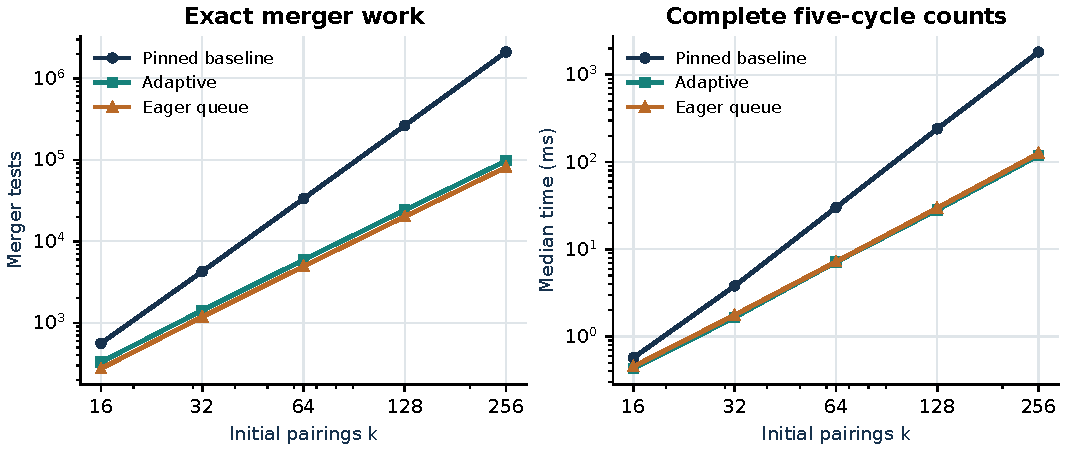
\includegraphics[width=\textwidth]{figures/five_cycle.pdf}
\caption{Exact merger work and complete-count time on the proved family.
Both axes are logarithmic. The curves illustrate the cubic versus quadratic
merger counts; the exponent claim comes from the proof, not curve fitting.}
\label{fig:five-cycle}
\end{figure}

Increasing the translation base to create longer integers leaves the
combinatorial trace pattern unchanged.  At 32 pairings and 66, 1,026, or
4,098 bits for $N$, all cases still take five cycles, with 4,260 old tests,
1,425 adaptive tests, and 1,186 eager tests.  The adaptive paired gains are
2.35, 2.64, and 2.72 respectively; arithmetic is included in elapsed time.
\begin{table}[htbp]
\centering
\small
\begin{tabular}{rrrrr}
\toprule
Bits of $N$ & Old ms & Adaptive ms & Queue ms & Paired gain \\
\midrule
66 & 4.721 & 2.003 & 2.019 & 2.35 \\
1026 & 7.401 & 2.814 & 2.669 & 2.64 \\
4098 & 16.278 & 5.989 & 5.245 & 2.72 \\
\bottomrule
\end{tabular}
\caption{Fixed 32-pairing, five-cycle instances with increasing endpoint bit length.}
\label{tab:binary}
\end{table}


\subsection{Easy inputs and native geometry}

An eager queue can be expensive when the first available pair always merges.
It evaluates $(k-1)^2$ candidates where the restart scan needs only $k-1$.
At 256 duplicate pairings, its median is 189.053 ms versus 1.109 ms for the
baseline.  This is why queue mode is an experimental option and the bounded
adaptive policy is the default.

An initial adaptive implementation also rebuilt the full periodic index
list after every immediate success.  Profiling exposed that avoidable cost
and motivated the lazy first-pair path in the delivered implementation.
The final easy-input measurements in \cref{tab:easy} place the adaptive
path close to the baseline; paired gains range from 0.945 to 1.022 across
the four cases.  A gain below one is a measured slowdown.  The new default
does not promise universal speedup.
\begin{table}[htbp]
\centering
\small
\begin{tabular}{rrrrrr}
\toprule
$k$ & Tests: old/adaptive & Old ms & Adaptive ms & Queue ms & Paired gain \\
\midrule
16 & 15 & 0.072 & 0.074 & 0.561 & 0.98 \\
64 & 63 & 0.275 & 0.287 & 9.916 & 0.96 \\
128 & 127 & 0.572 & 0.570 & 42.696 & 1.02 \\
256 & 255 & 1.109 & 1.131 & 189.053 & 0.94 \\
\bottomrule
\end{tabular}
\caption{Easy duplicate inputs. All adaptive runs complete without a queue switch.}
\label{tab:easy}
\end{table}


For native geometry, layered solid-torus meridian systems range from 4 to
128 tetrahedra.  Their normal coordinates and interval endpoints grow in
binary size with the layering.  The adaptive path performs exactly the
same number of merger tests as the old implementation and never switches
to the queue.  Its gain comes from indexing periodic rows once after a
failed first pair and avoiding repeated inner visits to nonperiodic rows.
At 128 tetrahedra, the median paired gain is 1.51, with median times
886.982 ms and 593.443 ms.  The smallest case is slightly slower.
\begin{table}[htbp]
\centering
\small
\begin{tabular}{rrrrrrr}
\toprule
$t$ & $k$ & Bits of $N$ & Cycles & Old ms & Adaptive ms & Paired gain \\
\midrule
4 & 18 & 6 & 9 & 0.337 & 0.339 & 0.97 \\
8 & 34 & 8 & 13 & 0.978 & 0.952 & 1.03 \\
16 & 66 & 14 & 21 & 4.365 & 3.932 & 1.11 \\
32 & 130 & 25 & 37 & 21.056 & 17.369 & 1.22 \\
64 & 258 & 47 & 69 & 130.881 & 95.281 & 1.35 \\
96 & 386 & 69 & 101 & 388.928 & 267.030 & 1.44 \\
128 & 514 & 92 & 133 & 886.982 & 593.443 & 1.51 \\
\bottomrule
\end{tabular}
\caption{Complete interval counts on native layered-solid-torus meridian arc systems.}
\label{tab:native}
\par\smallskip\footnotesize Geometry is constructed before timing. There are no adaptive queue switches and no changes in merger-test count in these cases.
\end{table}

\begin{figure}[htbp]
\centering
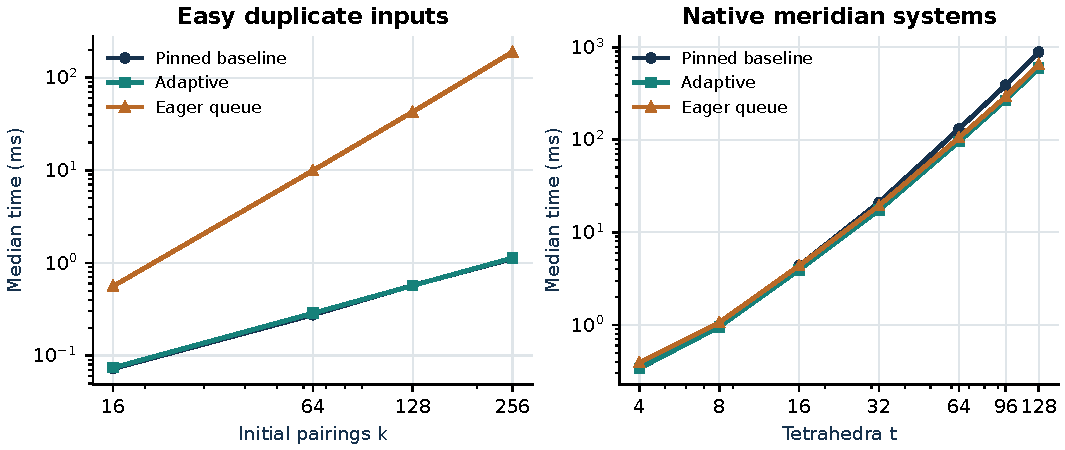
\includegraphics[width=\textwidth]{figures/easy_and_native.pdf}
\caption{The adaptive policy avoids the eager queue's large easy-input
cost. Native meridian systems show more modest gains without a queue switch.
Both axes are logarithmic; these are separate input families.}
\label{fig:easy-native}
\end{figure}

Finally, \cref{tab:profile-costs} records whole native queries, including
fresh geometry validation, for the established aggregate topology interface
and the new five-coordinate component profile.  The new interface obtains
its disk predicates from one weighted orbit calculation and needs no
orientation-double query.  At 96 tetrahedra the observed medians are
547.781 ms and 359.843 ms.  The output contracts differ, so this is a cost
comparison rather than a same-task speedup claim.  It shows that the richer
component information is practical on these fixtures; it does not measure
the time required to discover a useful normal surface.
\begin{table}[htbp]
\centering
\small
\begin{tabular}{rrr}
\toprule
$t$ & Aggregate topology ms & Component profile ms \\
\midrule
4 & 1.183 & 1.182 \\
16 & 9.806 & 8.132 \\
32 & 38.328 & 29.382 \\
64 & 195.910 & 137.648 \\
96 & 547.781 & 359.843 \\
\bottomrule
\end{tabular}
\caption{Native query costs, including fresh geometry validation. The outputs differ.}
\label{tab:profile-costs}
\par\smallskip\footnotesize These are costs of two different interfaces, not a same-task speedup experiment.
\end{table}


\subsection{What the measurements support}

The strongest supported performance conclusion is the proved improvement
for complete counts on the explicit interval family.  The native cases
support a smaller practical gain and validate the geometry-to-orbit path.
The component audit supports the implementation of the new certificate
predicate, and the huge-multiplicity demo confirms that its interface stays
compressed.  No experiment here measures a complete new knot recognizer on
hard diagrams, and none establishes the candidate or hierarchy bounds
required for the quasi-polynomial objective.

\section{A precise route toward quasi-polynomial recognition}
\label{sec:research}

The new component predicate improves the value of each supplied normal
candidate.  A candidate may carry irrelevant closed or boundary-parallel
components, yet its useful disk is still detected.  The scheduler improves
one operation repeatedly used by that predicate.  To turn these gains into
a global complexity theorem, one must control how candidates and geometric
states are obtained, how many are visited, and how their bit sizes evolve.

\subsection{A conditional assembly statement}

The following formulation makes these obligations explicit.  It is a
research specification, not an assertion that its hypotheses have been
implemented.

\begin{proposition}[Conditional recognition through compressed candidates]
\label{prop:conditional-recognition}
Suppose an algorithm, on an $n$-crossing knot diagram $D$, constructs in
polynomial time a compact triangulation $E(D)$ and a checked correspondence
with its knot exterior.  Suppose a complete candidate procedure has the
following properties:
\begin{enumerate}
\item It visits at most $S(n)$ states, including unsuccessful branches, with
an encoded state-size bound $B(n)$.
\item Each transition, each normal-vector construction, and all bookkeeping
take time polynomial in $B(n)$, including all integer bit costs.
\item Its terminal acceptance condition is the presence of a compressing
disk among the components of a supplied admissible normal vector; a terminal
rejection certificate or an exhaustive termination theorem establishes
completeness of rejection.
\end{enumerate}
Then adding the component query gives an exact recognizer with time
$S(n)\operatorname{poly}(B(n))$, apart from the polynomial exterior
construction.  In particular, if $B(n)$ is polynomial and
$S(n)=2^{O((\log n)^a)}$ for a fixed $a\geq1$, the resulting bound is
quasi-polynomial.
\end{proposition}

\begin{proof}
The component query is polynomial in each encoded input.  Its positive
predicate is exactly the existence of a compressing-disk component, and
the verified exterior correspondence makes boundary compressibility
equivalent to the input being the unknot.  The assumed rejection theorem
rules out unvisited positive instances after termination.  Summing the
polynomial transition and query costs over all visited states gives the
bound.  No component multiplicity is expanded in this sum.
\end{proof}

The proposition also shows why a fast verifier alone is insufficient.
Normal coordinates of bounded bit size still range over a vast set; bounding
their encoding is not a bound on the number of candidates examined.  A
successful search heuristic does not supply the rejection theorem in the
third hypothesis.

Lackenby's hierarchy iteration expression $L(g+1)^L$ provides a more
geometric target \cite{Lackenby2026}.  If $g\leq n^c$ and all operations
and state encodings satisfy polynomial bounds, then
\[
 \log\bigl(L(g+1)^L\bigr)=O(\log L+L\log n).
\]
Thus $L=O(\log n)$ would give $2^{O((\log n)^2)}$, while
$L=O((\log n)^2)$ gives $2^{O((\log n)^3)}$.  The latter agrees with the
exponent displayed in the 2021 Oxford handout \cite{Lackenby2021}.
The expression becomes a runtime bound only after the geometric operations,
branch count, and representation sizes have been bounded constructively.
It is not enough to count hierarchy levels while allowing an exponential
triangulation expansion inside a level.

\subsection{Research questions with concrete completion criteria}

\paragraph{1. Certify the passage from a diagram to a compact exterior.}
Can a diagram-to-triangulation constructor emit a short, independently
checkable correspondence including the peripheral marking?  The immediate
deliverable should be a source-bound certificate whose verification accepts
exactly the claimed exterior, with a proved polynomial tetrahedron and bit
bound.  This closes the first missing logical link before the new component
predicate can affect the ordinary recognizer.

\paragraph{2. Find candidates without enumerating all admissible vectors.}
Which hierarchy or handle moves produce a complete family of useful normal
vectors while visiting only quasi-polynomially many states?  The component
predicate permits extra disconnected summands, potentially relaxing the
candidate specification.  A useful theorem would show that a cheaply
constructed larger surface must contain the desired disk, without requiring
enumeration of every fundamental or vertex normal surface.  Any such theorem
must cover unsuccessful inputs as well as successful examples.

\paragraph{3. Recover a selected component in compressed coordinates.}
Given a positive five-coordinate profile, can one produce one actual disk
component and its $7t$ normal-coordinate vector in polynomial bit time?
One candidate approach first filters with five weights, then replays the
same orbit trace with one coordinate for each normal-piece type and suitable
representative information.  Classical weighted AHT makes the coordinate
payload plausible, but selecting a particular component inside a repeated
profile group and certifying its relation to the source remain explicit
tasks.  Returning all exponentially many components is not a suitable
completion criterion.

\paragraph{4. Preserve three-dimensional information through cutting.}
Can a verified disk or hierarchy surface be cut out while retaining a
polynomial representation of the residual manifold, parallelity regions,
peripheral curves, and attaching maps?  Scalar weights or set-incidence
profiles do not contain cyclic order or three-dimensional gluing data.
The compressed cutting and parallelity framework in
\cite[Theorem~14.4]{Lackenby2026} is a natural target for constructive
implementation and bit-size accounting.  A complete step should include
both an output representation and a checker for its geometric meaning.

\paragraph{5. Obtain a useful global potential.}
What potential controls hierarchy length, candidate branching, coordinate
growth, and the work of unsuccessful reductions simultaneously?  Existing
local simplifications can decrease a word length while increasing another
representation.  A successful potential should yield a recurrence for total
work, not merely demonstrate progress in one favorable parameter.  The
parameters $g$ and $L$ should be connected to quantities computed from the
input, with every representation conversion included.

\paragraph{6. Realize or exclude the cubic family in surface geometry.}
The five-cycle family proves an asymptotic improvement for legal interval
systems.  Does a comparable family arise from valid normal coordinates on
compact torus-boundary triangulations, preferably from verified knot
exteriors?  Alternatively, do geometric arc systems satisfy a structural
restriction that rules it out and yields a stronger scheduling theorem?
Either outcome would clarify which worst cases matter to the intended
recognizer.  The present native meridian measurements show smaller constant
factor gains and do not answer this question.

\paragraph{7. Reduce the event queue's memory without losing its theorem.}
Can one find all potentially successful periodic mergers using
$o(k^2)$ stored candidates while retaining a proved $O(k^2)$ or better
arithmetic work bound?  A naive per-row minimum can become invalid when a
candidate is deleted and can silently restore repeated full scans.  Useful
approaches must specify how failed pairs are remembered, how generation
changes are propagated, and how all rescans are amortized.  The full
trace-order guarantee is valuable, but a different order is acceptable only
with a renewed trace-length and correctness analysis.

\paragraph{8. Tune adaptive scheduling using measurable work.}
The bounded prelude already protects easy first-pair successes from eager
queue initialization.  What inexpensive indicators predict when building
the queue will pay for its memory and arithmetic costs?  The preliminary
experiment exposed a separate periodic-index rebuild cost, leading to the
lazy first-pair path included here.  Future policies should retain a
mathematical test allowance and be evaluated with paired timings on easy,
native, adversarial, and large-bit inputs.  Universal speedup should not be
assumed from a worst-case improvement.

\paragraph{9. Stream weighted replay and share geometric preparation.}
Can the producer emit checked operations to an online weight accumulator,
while also saving a replayable certificate, to avoid retaining redundant
state?  Can repeated candidates reuse a validated triangulation and the
boundary basis without trusting stale source data?  The desired output is a
clear ownership and source-binding contract, together with a peak-memory
bound.  These changes can improve practical searches without changing the
global mathematical exponent.

\paragraph{10. Extend component features only when they answer a needed
question.}
Which constant-dimensional additive predicates suffice for subsequent
hierarchy choices?  Euler characteristic and two mod-two evaluations suffice
for the torus compressing-disk predicate, but they do not recover slopes,
boundary-circle partitions, or embeddings.  Additional integer or oriented
weights may recover some of this information; nonadditive information may
require a richer compressed structure.  Each added field should have an
explicit interpretation, bit bound, and independent test.

\paragraph{11. Understand the higher-genus boundary obstruction.}
For genus $h>1$, $2h$ mod-two coordinates detect a nonzero boundary homology
class but miss essential separating curves.  Therefore replacing two cycles
by $2h$ cycles does not extend the disk-essentiality theorem.  Can a
compressed simple-curve algorithm decide essentiality for a selected disk
boundary while preserving source markings?  A completion criterion must
handle separating curves, multiple boundary components, and their
interaction with the chosen component, rather than only aggregate homology.

\paragraph{12. Shrink and verify the trusted geometric core.}
The current trace verifier is independent of scheduling, whereas geometric
preparation and weight construction are shared.  A second implementation or
a formal proof should target local edge orientation transport, the
one-cell/one-corner allocation, boundary homology bases with repeated
incidences, and full-range weight transfer.  The fixed Regina fixtures and
literal finite oracles are useful regression evidence, not substitutes for
these proofs.  Formalization should be accompanied by encoding and bit-cost
lemmas so that correctness does not conceal expansion.

\subsection{Recommended next integration sequence}

The most useful immediate sequence is to integrate the proved scheduler and
component query, add a certified exterior constructor, and recover a single
positive component in normal coordinates.  Those steps produce an exact
geometric acceptance path with inspectable evidence.  In parallel, a
hierarchy prototype should instrument state count, bit growth, parallelity
compression, and unsuccessful branches.  Its purpose is to test and refine
the hypotheses of \cref{prop:conditional-recognition}; small experimental
state counts should not be reported as a quasi-polynomial proof.

The long-term mathematical bottleneck is the controlled global geometric
search.  The present work removes avoidable repeated merger tests and
enriches the compressed certificate available at each candidate.  It makes
that bottleneck more explicit and gives subsequent research a stronger,
tested local interface.

\appendix
\section{Reproduction and repository integration}
\label{app:reproduction}

The archive is a self-contained research continuation, with the following
layout relative to its top-level directory:
\begin{center}
\begin{tabular}{p{0.28\textwidth}p{0.63\textwidth}}
\toprule
Path & Contents \\
\midrule
\path{article/} & This PDF, its main \TeX{} source, sections, bibliography,
generated tables, vector figures, and build instructions. \\
\path{code/fast/} & Runnable maintained source snapshot with the new modules,
tests, and dependency-free demonstration. \\
\path{code/reports/} & Minimal pinned archived oracle dependencies needed by
the complete maintained test suite. \\
\path{reference/} & Exact pinned historical interval producer used for
paired baseline measurements. \\
\path{experiments/} & Timing driver, independent component audit and frozen
trefoil fixture, and table/figure generator. \\
\path{results/} & Final raw measurements, finite-audit records, test log,
weighted-test summary, and concise demonstration output. \\
\path{integration.patch} & Changes to production code, tests, demonstration,
and the maintained README, with paths relative to the ProveIt repository. \\
\path{PROVENANCE.json} & Source pin, file identities, environment information,
and evidence-to-command mapping. \\
\bottomrule
\end{tabular}
\end{center}

The runtime source and demonstration require Python 3.10 or later; the
recorded environment uses 3.12.14.  The complete independent surface audit
requires Regina; the project already specifies its optional Regina range
in \path{code/fast/pyproject.toml}.  Plot regeneration requires Matplotlib.
PDF compilation uses a standard \LaTeX{} installation with pdf\LaTeX{},
Bib\TeX{}, Latin Modern, \code{microtype}, \code{cleveref}, and the packages
listed in the main source.  No external file download is required to read
the article, run the demonstration, or compare the supplied interval code.

From the archive root, the convenience driver exposes the independent jobs:
\begin{verbatim}
python reproduce.py demo
python reproduce.py tests
python reproduce.py audit
python reproduce.py benchmark
python reproduce.py figures
python reproduce.py article
\end{verbatim}
Regenerated outputs are written under \path{rerun/}, leaving the recorded
evidence intact.  Timings should be collected without concurrent heavy
jobs.  Repeated runs may change elapsed times while leaving operation
counts, component predicates, and certificate checks identical.

The benchmark command compares the delivered source to
\path{reference/interval_orbits.py}; it does not fetch a moving branch.
The independent normal audit reads the adjacent frozen trefoil fixture and
enumerates only the explicitly described finite families.  The weighted
test suite writes its small diagnostic JSON into the research folder, which
the convenience driver copies into the rerun results.  The driver reports
subprocess failure instead of silently continuing to a successful summary.

Before integrating code into another checkout, run
\begin{verbatim}
git apply --check /path/to/integration.patch
git apply /path/to/integration.patch
\end{verbatim}
from the ProveIt root.  The patch targets the pinned commit; later
concurrent changes may require ordinary review and conflict resolution.
The archive's source snapshot is useful for reproduction, but replacing
the whole current \path{fast/} directory with it would discard later work.
For the manuscript, copy \path{article/} as a complete subdirectory, for
example under
\path{Topology/UnknotRecognition/synthesis/component_certificates_20261009/}.
Its relative section, table, figure, and bibliography paths then remain valid.

The new production sources follow the maintained MIT No Attribution license.
Existing source and archived oracle license notices are retained.  The
bundle references third-party papers bibliographically; it does not
redistribute their downloaded PDFs.  The recorded raw results are evidence
for this continuation, while the proofs and source comments state the
generality and limits of each claim.

\begingroup
\raggedright
\phantomsection
\addcontentsline{toc}{section}{References}
\bibliographystyle{plain}
\bibliography{references}
\endgroup
\end{document}
